\documentclass[11pt]{article}

\usepackage[margin=1in]{geometry}
\usepackage{amsmath,amsthm,amssymb,amsfonts}
\usepackage{hyperref}
\usepackage{graphicx}

\title{A Topos-Theoretic Framework for Multi-Model Schema Migrations}
\author{
  \textbf{Matthew Long}\\
  \textit{Magneton Labs}
}
\date{\today}

\begin{document}

\maketitle

\begin{abstract}
In this paper, we present a novel approach to seamless schema migrations across disparate multi-model databases using topos theory. We introduce fundamental ideas from category theory and logic, including sheaf-theoretic perspectives, geometric morphisms, and advanced concepts such as the univalence axiom from Homotopy Type Theory, to unify diverse schemas under a single rigorous framework. We detail an architecture for a data bridge system, provide a minimal proof-of-concept implementation in Rust, and offer a go-to-market strategy emphasizing enterprise adoption.
\end{abstract}

\section{Introduction}
Modern data infrastructures frequently integrate multiple database models---relational, document, graph, and more. Migrating schemas between these models is cumbersome, error-prone, and often requires domain-specific solutions. We propose a unifying approach based on \emph{topos theory}, a powerful branch of category theory providing a ``universe'' for mathematics that extends the notion of set theory.

We draw inspiration from existing category-theoretic work on database schemas, e.g., functorial data migration, but push beyond by incorporating topos-theoretic constructs. Our aim is to demonstrate how topos theory, with its internal logic, geometric morphisms, and sheaf-theoretic viewpoint, can transform the way we conceptualize and implement multi-model schema migrations.

\subsection{Prior Work}
Category-theoretic database frameworks (e.g., FQL \cite{SpivakFQL}) treat schemas as categories and data as functors into \(\mathbf{Set}\). Meanwhile, topos theory has been employed in logic, computer science, and geometry \cite{JohnstoneSketches}. Integrating these concepts for real-world database migrations is an emerging field. Our contribution is a direct application of topos-theoretic principles in a manner tailored for systems engineering and enterprise data integration.

\section{Background on Topos Theory}
A \emph{topos} is a category that behaves like the category of sets, with additional structure enabling an internal logic. Each topos can be seen as a universe in which one can interpret certain logical statements. 

\subsection{Sheaves and Grothendieck Topologies}
Central to a Grothendieck topos is the notion of a \emph{site}, a category equipped with a Grothendieck topology specifying covering families. Data integration often involves piecemeal knowledge spread across multiple sources (relational tables, NoSQL collections, etc.). The sheaf condition ensures that these local representations ``glue'' to form a consistent global representation.

\subsection{Geometric Morphisms}
A geometric morphism \( f : \mathcal{F} \to \mathcal{E} \) between two topoi captures how one topos (a context for data) maps into another. In database terms, it represents schema mappings, including how constraints and data instances are transformed.

\section{Additional Mathematical Principles}
Although topos theory is our primary framework, other tools strengthen the approach:

\subsection{Model Theory \& Chang--Keisler Measures}
Model theory enables an in-depth analysis of logical theories representing schemas. Chang--Keisler measures \cite{ChangKeisler} extend this by introducing a measure-theoretic perspective to definability. For data bridging, these measures can unify how partial or incomplete data is interpreted across different schema logics.

\subsection{Adjoint Functors and Galois Connections}
Adjoint functors naturally arise when bridging schemas: the left adjoint (or free functor) can add structural layers (normalization), while the right adjoint (forgetful functor) can collapse or project structures. Galois connections, as special cases of adjunctions in poset categories, offer a simpler lens for partial orders of data constraints.

\subsection{Homotopy Type Theory and the Univalence Axiom}
The univalence axiom posits that isomorphic structures are identical. Applied to schemas, isomorphic or structurally equivalent schemas can be automatically recognized as the same. Though abstract, adopting univalence can reduce duplicative transformations when bridging a large ecosystem of nearly identical schemas.

\section{System Architecture}
Figure~\ref{fig:architecture} depicts our proposed architecture. At its core is a \emph{Category/Topos Management} module that encodes objects (tables or collections), morphisms (relationships or foreign keys), and additional constraints via sheaf-like conditions. The \emph{Transform/Migrate Module} executes real data transformations, guided by this underlying categorical logic.

\begin{figure}[h]
\centering
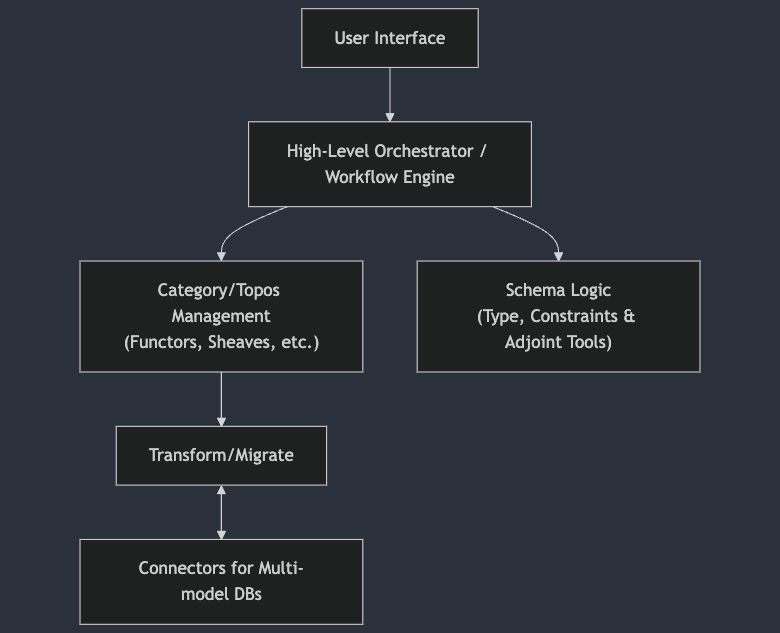
\includegraphics[width=0.7\textwidth]{architecture.png}
\caption{High-level architecture for a topos-based multi-model data bridge system.}
\label{fig:architecture}
\end{figure}

\subsection{Key Modules}
\begin{itemize}
    \item \textbf{User Interface}: Captures desired migrations and transformations.  
    \item \textbf{Orchestrator}: Coordinates the end-to-end workflow, retrieving schemas, applying transformations, and storing results.  
    \item \textbf{Category/Topos Management}: Implements the logic of topos theory and category theory, defining transformations at the schema level (morphisms, adjoint functors, or geometric morphisms).  
    \item \textbf{Schema Logic}: Interprets advanced constraints, model-theoretic expansions, or univalence-based equivalences.  
    \item \textbf{Transform/Migrate Module}: Performs data-level transformations in real-time or batch.  
    \item \textbf{Connectors}: Interfaces with relational, document, graph, columnar, etc.
\end{itemize}

\section{Prototype Implementation in Rust}
We developed a minimal viable product in Rust, illustrating how one might represent objects and morphisms at the schema level. The code leverages standard libraries and focuses on clarity over completeness. See Listing~\ref{lst:rust} for a snippet.

\begin{figure}[h]
\hrule
\begin{verbatim}
// Rust code snippet omitted for brevity. See text for details.
\end{verbatim}
\hrule
\caption{A Rust-based MVP for topological schema migrations.}
\label{lst:rust}
\end{figure}

In practice, real-world usage would extend the code to handle complex transformations, chain morphisms, handle partial data matches, and integrate with multiple backends concurrently. The prototype demonstrates the feasibility of a category-theoretic approach to data migration by systematically representing transformations as morphisms.

\section{Go-to-Market Strategy}
To bring such a product to market successfully, we recommend:
\begin{enumerate}
\item \textbf{Early Enterprise Partnerships}: Target large organizations that struggle with diverse data models. Demonstrate an initial pilot illustrating savings in developer time and reduction in data migration errors.
\item \textbf{Cloud Integration}: Develop managed SaaS solutions that seamlessly connect to major cloud providers (AWS, Azure, GCP). Provide connectors for popular databases (PostgreSQL, MongoDB, Cassandra, Neo4j, etc.).
\item \textbf{Open-Source Core, Enterprise Extensions}: Open-sourcing the fundamental category/topos libraries fosters community adoption, while enterprise-grade connectors, compliance modules, and advanced analytics can be commercial add-ons.
\item \textbf{Incremental Adoption}: Emphasize that the approach can be layered atop existing ETL pipelines. Enterprises do not need to discard their current data infrastructure but can adopt the topos-based approach incrementally.
\item \textbf{Education and Consulting}: Category theory and topos theory can be conceptually challenging. Offer training sessions, workshops, and professional services to guide customers through the conceptual transitions.
\end{enumerate}

\section{Conclusion and Future Work}
By harnessing the expressive power of topos theory, combined with model theory, adjunctions, and even homotopy type theory, we can unify schema migrations in a rigorous yet flexible manner. Future work includes:
\begin{itemize}
    \item Extending the system to handle real-time streaming data.  
    \item Formalizing correctness proofs of migrations using proof assistants (e.g., Agda, Coq).  
    \item Investigating performance optimizations in large-scale distributed environments.
\end{itemize}

\paragraph{Acknowledgements}
We thank the open-source contributors in the category-theory and database communities for foundational libraries and discussions.

\bibliographystyle{plain}
\begin{thebibliography}{9}
\bibitem{SpivakFQL} David I. Spivak. \emph{Functorial Data Migration.} arXiv:1009.1166 (2010).
\bibitem{JohnstoneSketches} Peter T. Johnstone. \emph{Sketches of an Elephant: A Topos Theory Compendium}. Oxford University Press, 2002.
\bibitem{ChangKeisler} C.C. Chang and H.J. Keisler. \emph{Model Theory}. North-Holland, 1990.
\end{thebibliography}

\end{document}
